\documentclass[a4paper,12pt]{article}

\usepackage[spanish]{babel}
\usepackage{listings}
\usepackage[utf8]{inputenc}
\usepackage{titling}
\usepackage{enumitem}
\usepackage{fancyhdr}
\usepackage{xcolor}
\usepackage{geometry}
\usepackage{graphicx}
\usepackage{hyperref}
\usepackage{cite}
\usepackage{url}
\usepackage{fix-cm}
\usepackage{tikz}
\usepackage{etoolbox}
\usepackage[format=plain,
            labelfont={bf,it},
            textfont=it]{caption}
\usetikzlibrary{positioning}
\usetikzlibrary{arrows.meta}
\usetikzlibrary{calc}

\patchcmd{\thebibliography}{\section*{\refname}}{}{}{}

%%search -> (?:url=\{)(.*)(:?\})
%%replace -> howpublished={\\url{$1}}
%\geometry{a4paper, left=4em, right=4em, top=0em, bottom=4em}

\lstset{
    frame=single,
    breaklines=true,
    numbers=left,
    keywordstyle=\color{blue},
    numbersep=15pt,
    numberstyle=,
    basicstyle=\linespread{1.0}\selectfont\ttfamily,
    commentstyle=\color{gray},
    stringstyle=\color{orange},
    identifierstyle=\color{green!40!black},
}

\setlength{\parindent}{4em}
%%\setlength{\parindent}{0em}
\setlength{\parskip}{0.8em}
    
%%\renewcommand{\familydefault}{phv} %%Seleccionamos Helvetica
    
\lstdefinestyle{console}
{
    numbers=left,
    backgroundcolor=\color{violet},
    %%belowcaptionskip=1\baselineskip,
    breaklines=true,
    %%xleftmargin=\parindent,
    %%showstringspaces=false,
    basicstyle=\footnotesize\ttfamily,
    %%keywordstyle=\bfseries\color{green!40!black},
    %%commentstyle=\itshape\color{green},
    %%identifierstyle=\color{blue},
    %%stringstyle=\color{orange},
    basicstyle=\scriptsize\color{white}\ttfamily,
}

\newcommand{\size}[2]{{\fontsize{#1}{0}\selectfont#2}}
    
\title{Triángulo de Penrose}
%\subtitle{Diseño en 3D e implementación en OpenGL}
\date{}
\author{Aldán Creo Mariño}

\pagestyle{fancy}
\fancyhead[l]{Proyecto final}

\bibliographystyle{plain}
    
\begin{document}

\maketitle

\newpage
\tableofcontents
\newpage

\section{Concepto}
\subsection{El triángulo de Penrose}

El \textbf{triángulo de Penrose} es una figura imposible diseñada en 1934 por el artista sueco Oscar Reutersvärd. Sin embargo, no cobró notoriedad hasta 1954, cuando un matemático, Rodzher Penrouz (de ahí el nombre de la figura) escribió un artículo sobre figuras imposibles, que resultó muy llamativo. Desde ese momento pasó a formar parte de la cultura popular.

\begin{figure}
    \centering
    \resizebox*{0.4\textwidth}{!}{
    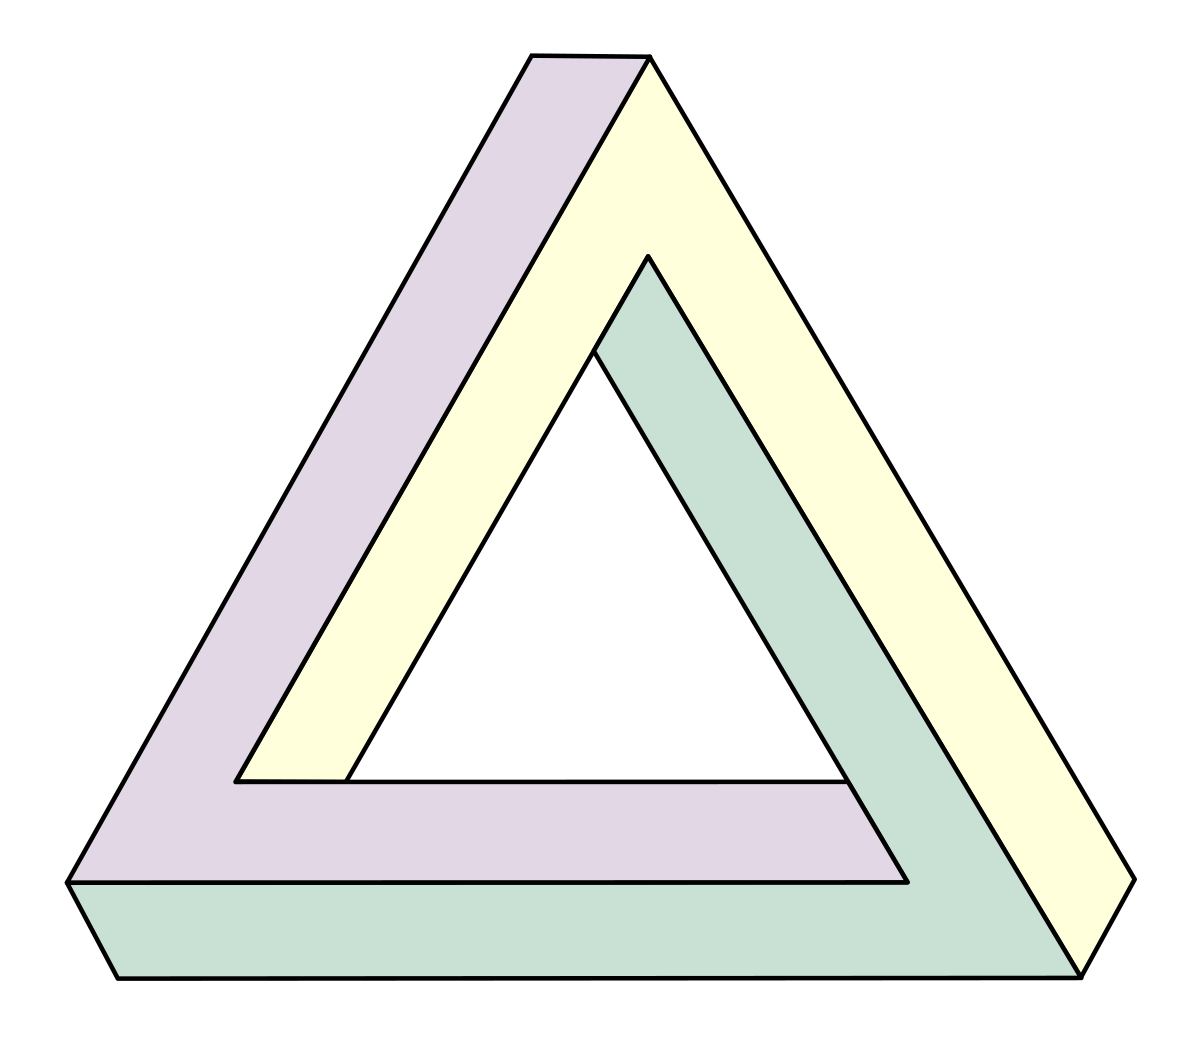
\includegraphics{1200px-Penrose_triangle.svg.png}
    }
    \caption{El triángulo de Penrose} \label{imagen_triangulo}
\end{figure}

La figura tiene el aspecto mostrado en \ref{imagen_triangulo}.

A nivel personal, me resultan especialmente fascinantes todos los temas relacionados con figuras imposibles, y por eso quería que mi proyecto de la asignatura girase en torno a ellas. El triángulo de Penrose me pareció la figura más icónica que existe, entre las figuras imposibles, y por eso he desarrollado mi proyecto sobre la misma.

\subsection{Idea base para el desarrollo}

Para hacer el desarrollo, me he basado en un juego de móvil llamado \textit{hocus} \cite{hocus}. El juego se basa en el uso de figuras imposibles, y concretamente tiene un nivel basado en el triángulo de Penrose, mostrado en \ref{nivel_hocus}.

\begin{figure}
    \centering
    \resizebox*{0.4\textwidth}{!}{
    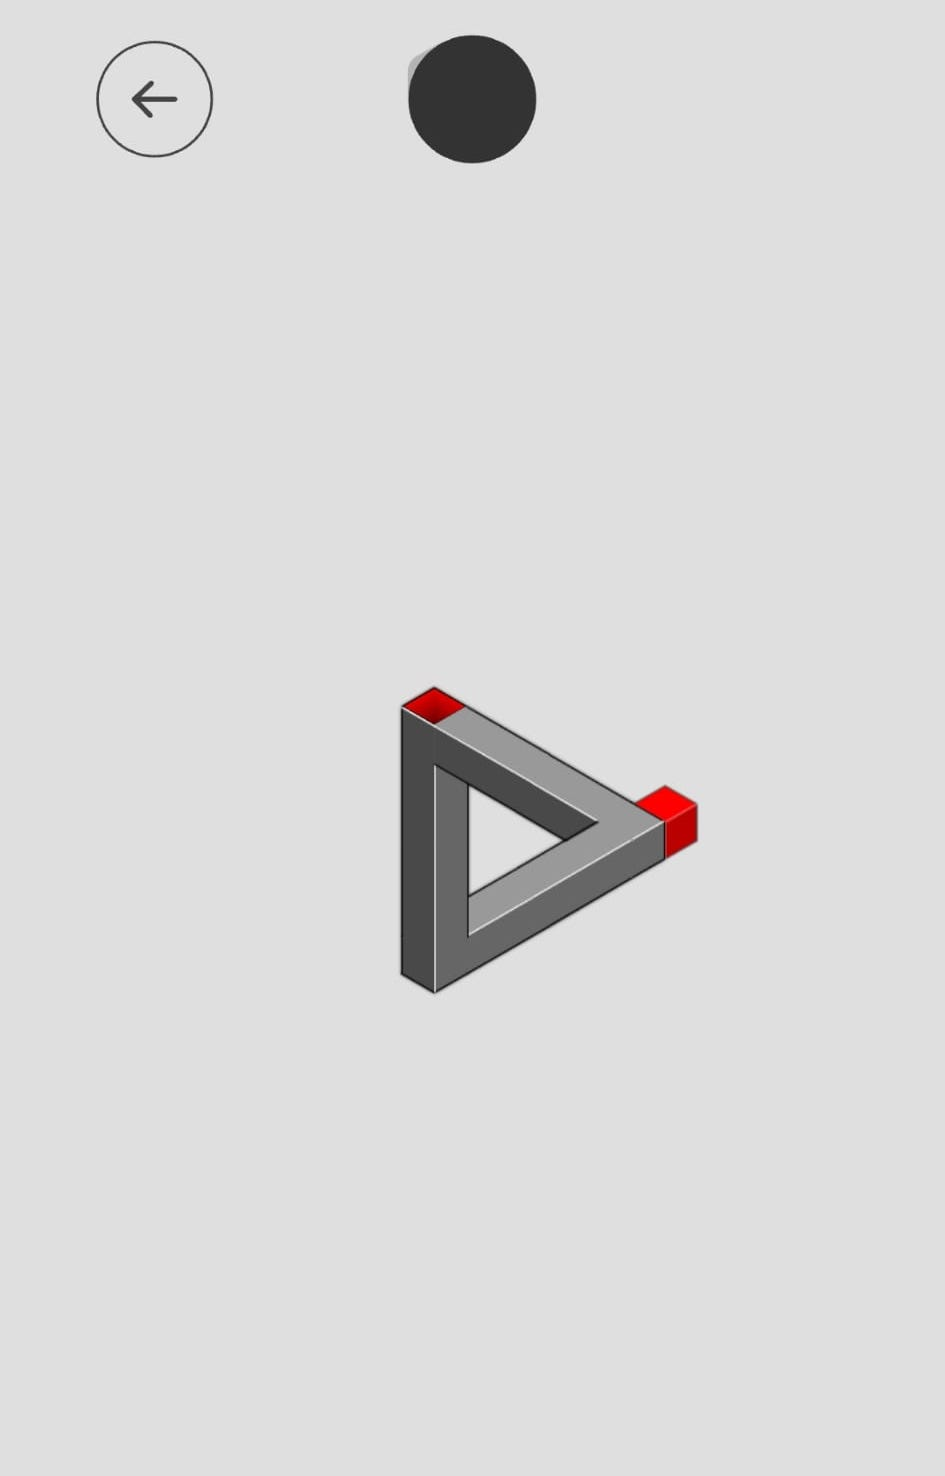
\includegraphics{hocus.jpeg}
    }
    \caption{Nivel 4 de \textit{hocus}} \label{nivel_hocus}
\end{figure}

\section{Diseño del modelo 3D}

\subsection{Obtención del modelo}

He comenzado con un modelo 3D disponible en \cite{modeloTriangulo}. Se trata de una página destinada a la impresión 3D, así que el modelo que ofrecían no era exactamente el apropiado para importar en la aplicación. Por eso tuve que editarlo de forma adecuada en Blender.

\subsection{Edición en Blender}

El modelo que descargué venía con todas las caras creadas, incluso las que en la aplicación aparecen ocultas. Esto, en principio, no debería suponer un problema, pero en la práctica sí lo es, cuando intento aplicar el algoritmo del pintor, que describiré en \ref{algoritmo_pintor}.

Por eso eliminé las caras ocultas del modelo, pasando de \ref{caras_ocultas_sin_borrar} a \ref{caras_ocultas_borradas}.

\begin{figure}
    \centering
    \resizebox*{0.8\textwidth}{!}{
    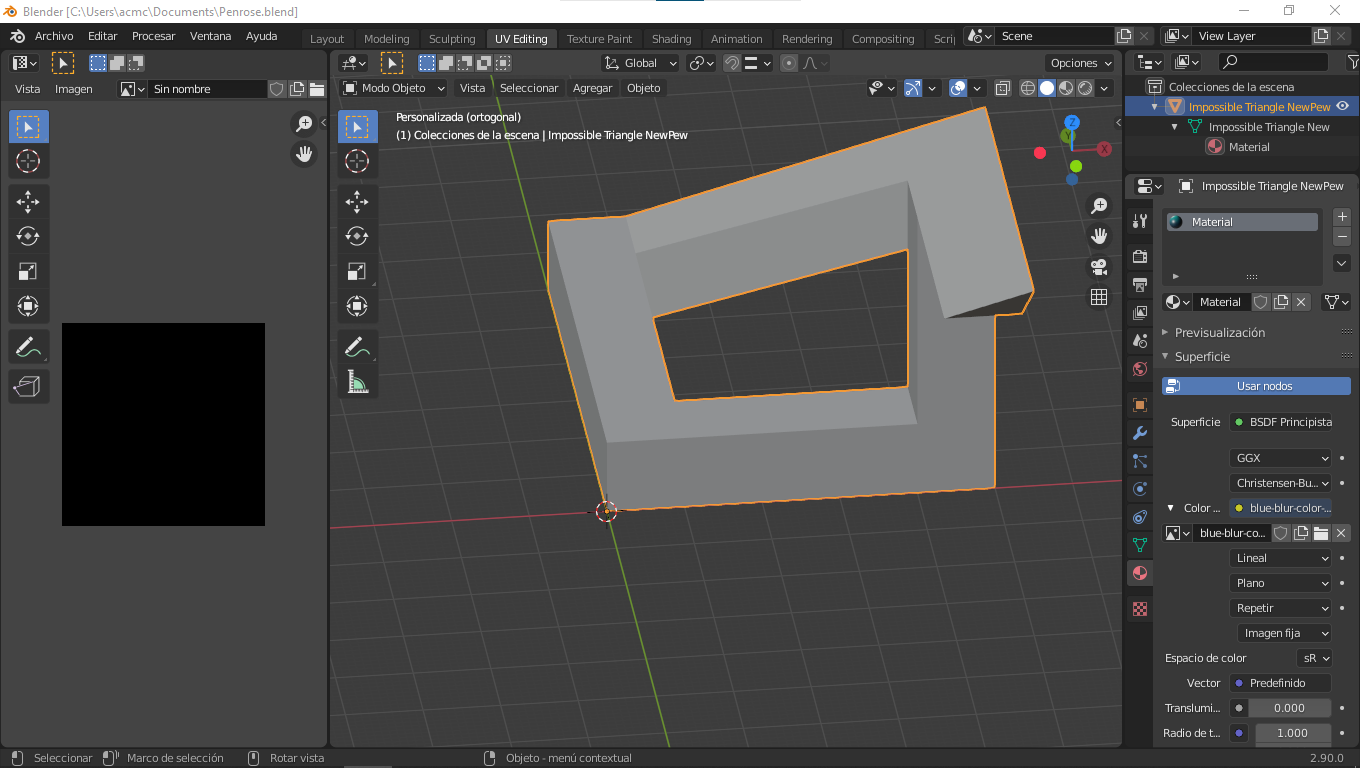
\includegraphics{caras_ocultas_sin_borrar.png}
    }
    \caption{Modelo original, con las caras ocultas sin borrar} \label{caras_ocultas_sin_borrar}
\end{figure}

\begin{figure}
    \centering
    \resizebox*{0.8\textwidth}{!}{
    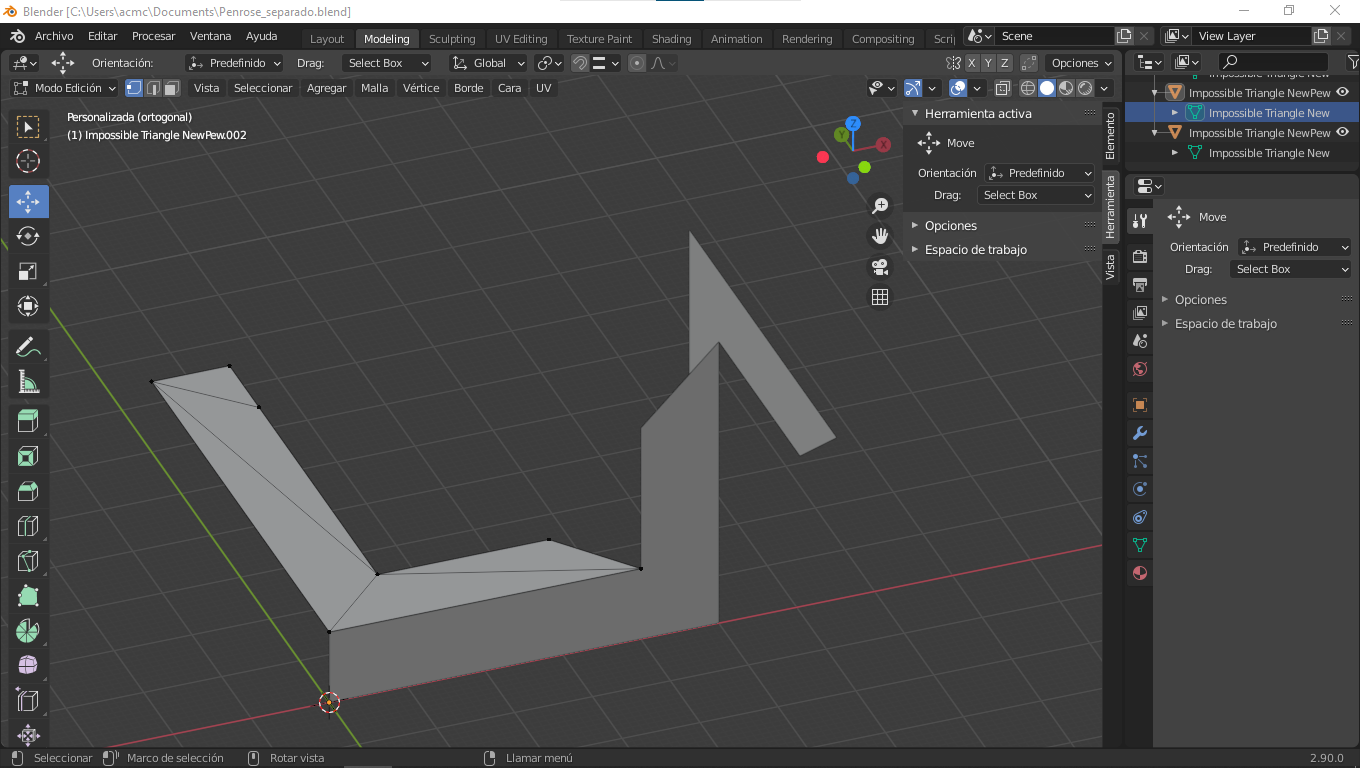
\includegraphics{caras_ocultas_borradas.png}
    }
    \caption{Modelo editado. Se han eliminado las caras ocultas y se ha separado en piezas.} \label{caras_ocultas_borradas}
\end{figure}

Además, separé las tres ``caras'' del triángulo, para poder aplicar después el algoritmo del pintor, según las secciones marcadas en rojo en \ref{separacion_caras_triangulo}. Es relevante comentar que, en este documento, llamo ``caras'' a cada una de las tres mallas que he separado, por simplicidad. Técnicamente son mallas compuestas de múltiples caras.

\begin{figure}
    \centering
    \resizebox*{0.6\textwidth}{!}{
    
\includegraphics{caras_marcadas.png}
    }
    \caption{Separación de la malla en tres, vista desde la aplicación. Los límites de las caras están marcados en rojo.} \label{separacion_caras_triangulo}
\end{figure}

También hice el mapeado UV de las mallas, en caso de que quisiera aplicarle una textura posteriormente. Finalmente, deseché esa idea, ya que me pareció que quedaría recargado y sería más elegante un color más plano, como se ve en la versión final de la aplicación. La textura decidí aplicarla a la esfera.

\section{Programación de la aplicación con OpenGL}
\subsection{Estructura del código}

\subsection{Importación del modelo del triángulo}

Desde Blender, exporté el modelo en formato \texttt{.obj}. Este formato permite leerlo de forma bastante directa desde OpenGL, pero tiene que ser procesado previamente. Mi primera intención sería intentar usar la librería de carga de modelos \texttt{Assimp}, que según leí en Internet es muy utilizada, pero como no estoy seguro de que esté permitido usar una librería externa en el proyecto, decidí procesar yo mismo el modelo para incorporarlo al código de la aplicación.

El formato del archivo es interpretable de forma bastante directa, así que utilicé expresiones regulares para convertir líneas de la forma \ref{lineas_obj} a vectores, como en \ref{lineas_obj_convertidas}.

\begin{figure}
    \centering
    \begin{minipage}[c]{0.7\textwidth}
        \begin{lstlisting}
f 1/2/3 2/3/3 3/4/3
        \end{lstlisting}
    \end{minipage}
    \caption{Línea del fichero \texttt{.obj} que describe una cara.} \label{lineas_obj}
\end{figure}
\begin{figure}
    \centering
    \begin{minipage}[c]{0.7\textwidth}
        \begin{lstlisting}
1, 2, 3, 2, 3, 3, 3, 4, 3,
        \end{lstlisting}
    \end{minipage}
    \caption{Línea convertida a formato vector de \texttt{unsigned int}s, para su uso directo en la aplicación. Corresponde a \ref{lineas_obj}.} \label{lineas_obj_convertidas}
\end{figure}

Utilicé el mismo procedimiento para todas las líneas, que son básicamente de cuatro tipos (vértices, caras, normales y texturizado).

De esta forma, construí un fichero \texttt{penrose.h}, basándome en el de las prácticas (\texttt{esfera.h}), con la información necesaria sobre la figura.

Pese a todo, como comentaba, realmente son tres mallas separadas, así que en el fichero de información solo incluí datos sobre vértices, normales y texturas, pero no sobre las caras, ya que dependen de cada malla. En el código de la aplicación lo que hago es incluir tres funciones, (\texttt{crearPenroseFrontal}, \texttt{crearPenroseLateral}, y \texttt{crearPenroseTrasero}), y dentro de cada función incluyo un vector con la información adecuada sobre las caras, que después se encarga de procesar un bucle dentro de la función para crear el \texttt{VAO} correspondiente. De esta forma, genera la información necesaria para que OpenGL pueda procesar la información del objeto.

Una operación importante que hace el bucle es decrementar en una unidad todas las referencias del vector, ya que el formato \texttt{.obj} utiliza indexado en base a 1, y en C los índices empiezan en 0. Es un aspecto importante, que me llevó cierto tiempo descubrir, ya que inicialmente no aplicaba esta operación, y por ello todos los vértices estaban mal referenciados, dando lugar a un dibujo como el recogido en la figura \ref{antes_de_corregir_indexado}.

\begin{figure}
    \centering
    \resizebox*{0.6\textwidth}{!}{
    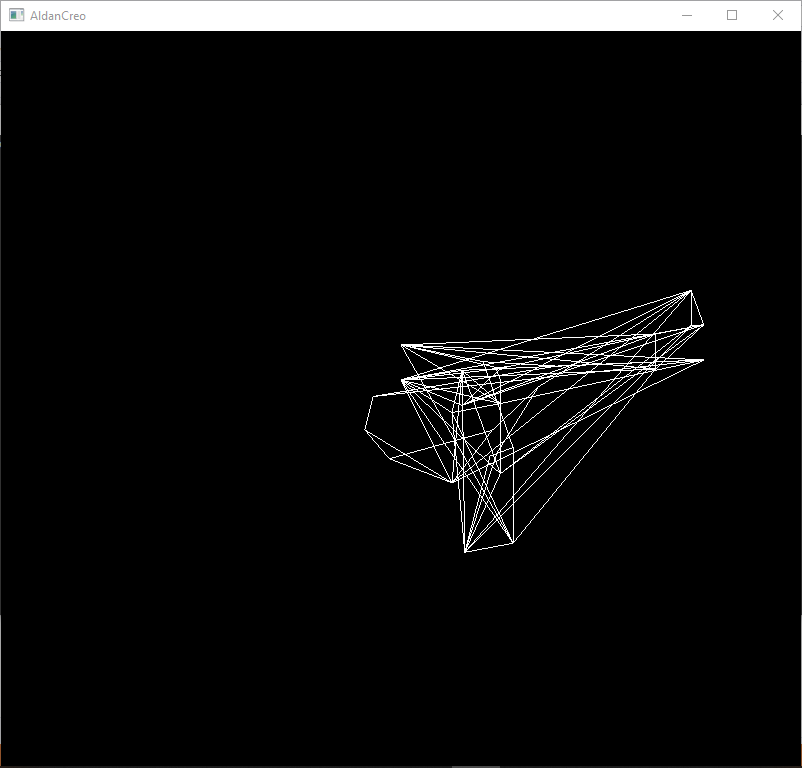
\includegraphics{Penrose_1_no_funciona.png}
    }
    \caption{Visualización de la aplicación en etapas previas del desarrollo, antes de tener en cuenta que el indexado de vértices, normales y texturas, en el formato \texttt{.obj}, empieza en 0.} \label{antes_de_corregir_indexado}
\end{figure}

\subsection{Iluminación}

\subsection{Texturizado}

\subsection{Algoritmo del pintor} \label{algoritmo_pintor}

\section{Comentarios finales}

\bibliography{export}

\end{document}